\documentclass{ximera}
\usepackage{sagetex}
\usepackage{multicol}
%% handout
%% space
%% newpage
%% numbers
%% nooutcomes

%% You can put user macros here
%% However, you cannot make new environments

\graphicspath{{./}{module1Activity/}{module2Activity/}{module3Activity/}}

\usepackage{sagetex}
\usepackage{tikz}
\usepackage{hyperref}
\usepackage{tkz-euclide}
\usetkzobj{all}
\pgfplotsset{compat=1.7} % prevents compile error.

\tikzstyle geometryDiagrams=[ultra thick,color=blue!50!black]
 %% we can turn off input when making a master document

\outcome{Understand and solve quadratic equations.}
\author{Darryl Chamberlain Jr.}
 
\title{Objective 2 - Graphing quadratic functions.}

\begin{document}
\begin{abstract}
Describe the salient characteristics of quadratic functions.
\end{abstract}
\maketitle

\href{https://cnx.org/contents/mwjClAV_@8.1:-Sm9he1Q@17/Quadratic-Functions}{Link to section in online textbook.}

%%%%%%%%%%%%%%%%%%%%%
%%%  Objective 1  %%%
%%%%%%%%%%%%%%%%%%%%%

First, watch 
\href{https://mediasite.video.ufl.edu/Mediasite/Play/b3664c4b8bbb458a969fecac7a80759c1d}{this video} to review the main characteristics of a quadratic function. Feel free to pause the video and fill out the notes as you go. 

Now practice working with converting between quadratic equations and their graphs below. 

\begin{question}
Write the equation of the graph presented below in the form $f(x)=ax^2+bx+c$, assuming $a=1$ or $a=-1$. 

\begin{center}
	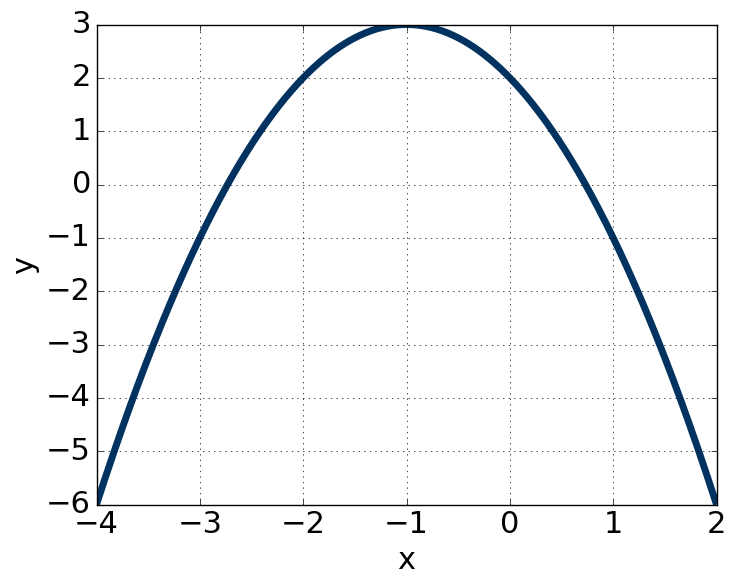
\includegraphics{question1Astatic.png}
\end{center}
% $-(x+1)^2+3 = -(x^2+2x+1)+3 = -x^2-2x+2 $
$y = \answer{-1} x^2 + \answer{-2} x + \answer{2}$
\end{question}

\begin{question}
Write the equation of the graph presented below in the form $f(x)=ax^2+bx+c$, assuming $a=1$ or $a=-1$. 

\begin{center}
	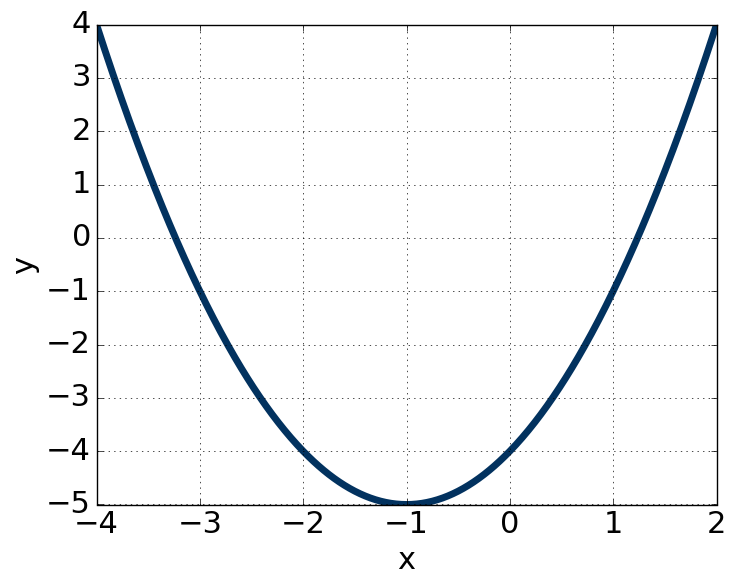
\includegraphics{question1Bstatic.png}
\end{center}

% $(x+1)^2-5 = x^2+2x+1-5=x^2+2x-4 $
$y = \answer{1} x^2 + \answer{2} x + \answer{-4}$
\end{question}

\begin{question}
Write the equation of the graph presented below in the form $f(x)=ax^2+bx+c$, assuming $a=1$ or $a=-1$. 

\begin{center}
	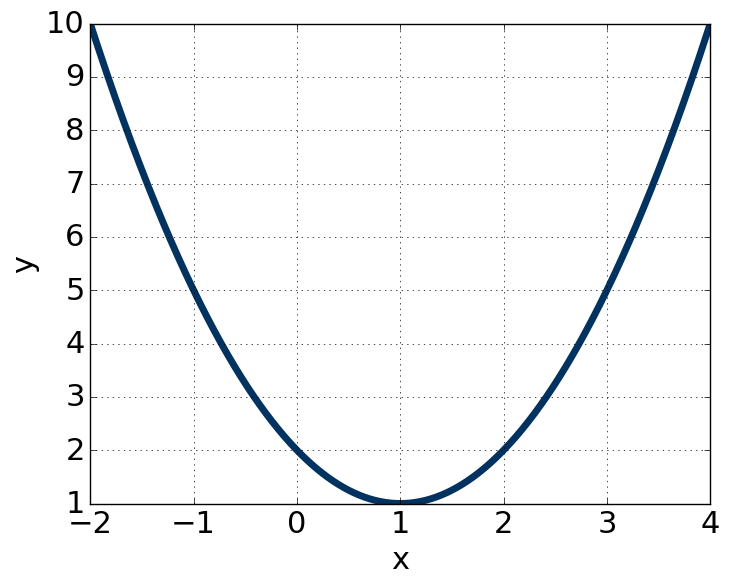
\includegraphics{question1Cstatic.png}
\end{center}

$y = \answer{1} x^2 + \answer{-2} x + \answer{2}$
\end{question}

\begin{question}
Graph the equation $f(x)= (x-3)^2-19. $

\begin{table}
\begin{tabular}{l l}
	\begin{tabular}{|c c|}
		\hline 
		& \\
		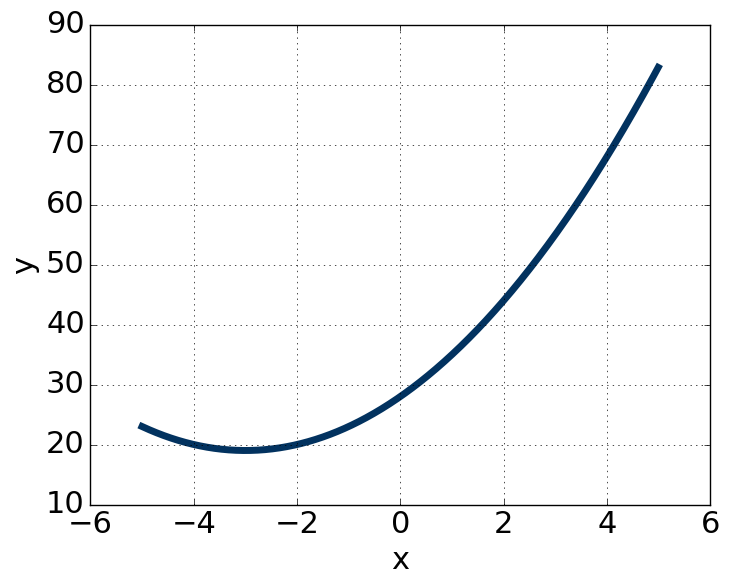
\includegraphics{question2Astatic.png} & Choice A \\   & \\ 
		\hline
		& \\
		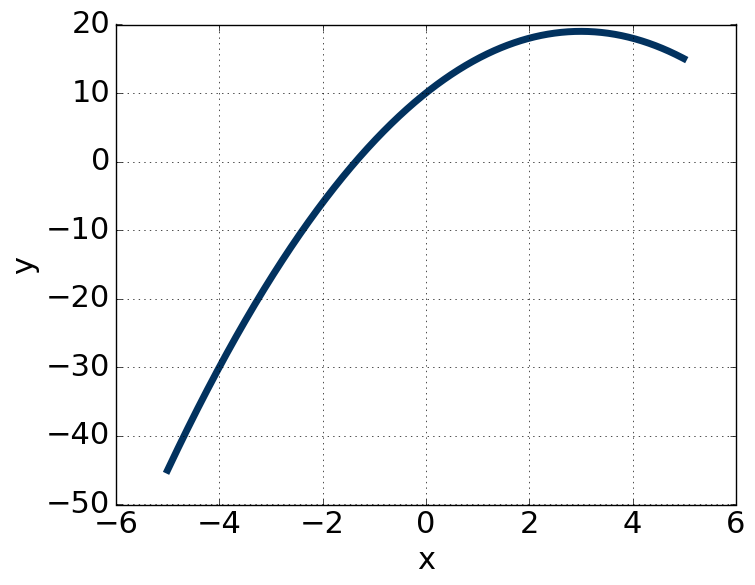
\includegraphics{question2Bstatic.png} & Choice B \\
		& \\
		\hline 
		& \\
		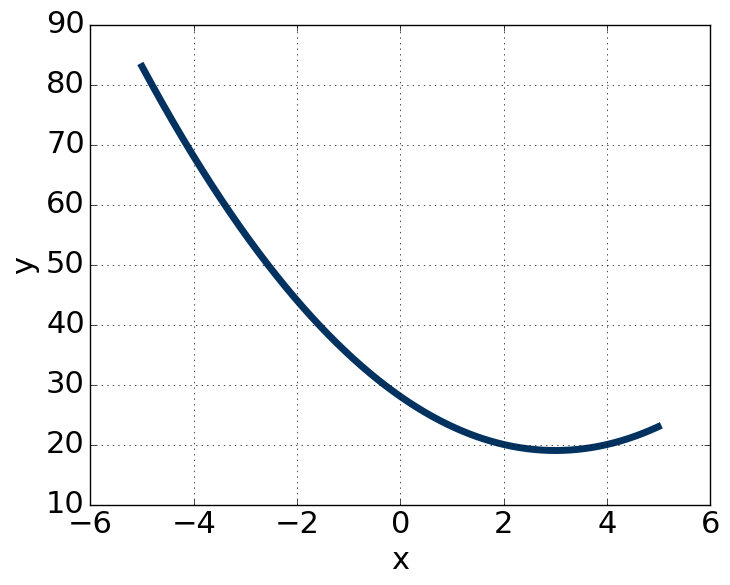
\includegraphics{question2Cstatic.png} & Choice C \\
		& \\
		\hline 
	\end{tabular}

	\begin{tabular}{|c c|}
		\hline
		& \\
		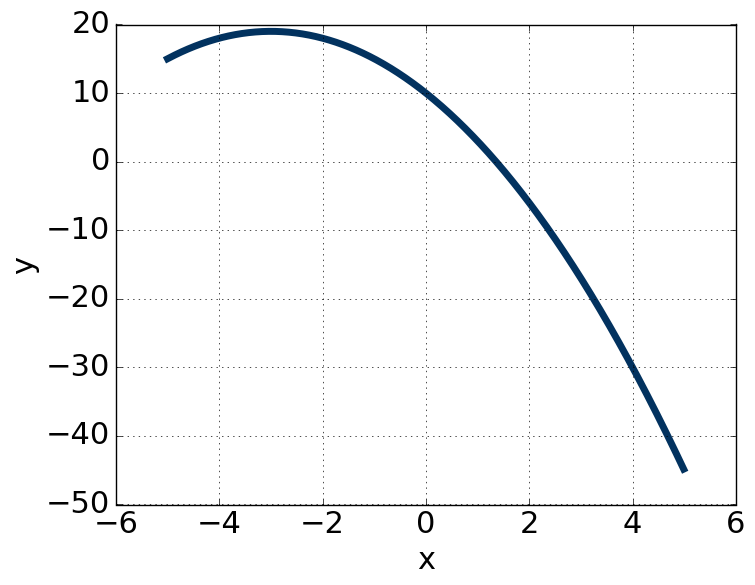
\includegraphics{question2Dstatic.png} & Choice D \\
		& \\
		\hline 
		& \\
		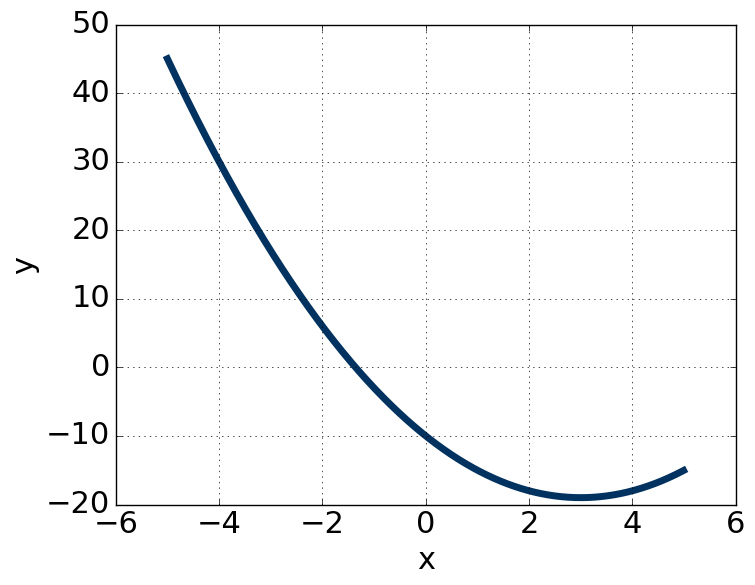
\includegraphics{question2Estatic.png} & Choice E \\
		& \\
		\hline 
	\end{tabular}
\end{tabular}
\end{table}


\begin{multipleChoice}
    \choice A
    \choice B
    \choice C
    \choice D
    \choice[correct] E
\end{multipleChoice}

\end{question}

\textbf{Since Xronos does not like making dynamic graphs, we can't practice questions like we could see on the exam perfectly. The questions below will do similar things you could see on the exam that you can practice.}

\begin{sagesilent}
def maybeMakeNegative(natural):
    integer = natural*(-1)**ZZ.random_element(2)
    return integer
#
def createVertexAndEquation(direction): 
    vx = maybeMakeNegative(ZZ.random_element(2, 10))
    vy = maybeMakeNegative(ZZ.random_element(2, 10))
    equationCoefficients = [direction, -direction*2*vx, direction*(vx)**2 + vy]
    vertex = [vx, vy]
    extraX = maybeMakeNegative(ZZ.random_element(2, 7))
    extraY = equationCoefficients[0]*(extraX)**2 - 2*direction*vx*extraX + direction*(vx)**2+vy
    extraPoint = [extraX, extraY]
    return [vertex, equationCoefficients, extraPoint]
########
### QUESTION 1 ###
direction1 = 1
vertex1, equationCoefficients1, extraPoint1 = createVertexAndEquation(direction1)
### QUESTION 2 ###
direction2 = -1
vertex2, equationCoefficients2, extraPoint2 = createVertexAndEquation(direction2)
### QUESTION 3 ###
direction3 = maybeMakeNegative(ZZ.random_element(2, 10))
vertex3, equationCoefficients3, extraPoint3 = createVertexAndEquation(direction3)
\end{sagesilent}

\begin{exercise}
	Given the quadratic function has the vertex at $(\sage{vertex1[0]}, \sage{vertex1[1]})$ and is pointing up, construct the equation of the function. Assume $a=1$ or $a=-1$. 
	
	$$f(x) = \answer{\sage{equationCoefficients1[0]}}x^2 + \answer{\sage{equationCoefficients1[1]}}x + \answer{\sage{equationCoefficients1[2]}}$$
	
	\begin{hint}
		To get started, write the equation in vertex form. Then, be careful as you multiply out. 
	\end{hint}
	
\end{exercise}

\begin{exercise}
	Given the quadratic function has the vertex at $(\sage{vertex1[0]}, \sage{vertex1[1]})$ and is pointing up, construct the equation of the function. Assume $a=1$ or $a=-1$. 
	
	$$f(x) = \answer{\sage{equationCoefficients1[0]}}x^2 + \answer{\sage{equationCoefficients1[1]}}x + \answer{\sage{equationCoefficients1[2]}}$$
	
	\begin{hint}
		To get started, write the equation in vertex form. Then, be careful as you multiply out. 
	\end{hint}
	
\end{exercise}

\begin{exercise}
	Given the quadratic function has the vertex at $(\sage{vertex2[0]}, \sage{vertex2[1]})$ and is pointing down, construct the equation of the function. Assume $a=1$ or $a=-1$. 
	
	$$f(x) = \answer{\sage{equationCoefficients2[0]}}x^2 + \answer{\sage{equationCoefficients2[1]}}x + \answer{\sage{equationCoefficients2[2]}}$$
	
	\begin{hint}
		To get started, write the equation in vertex form. Then, be careful as you multiply out. 
	\end{hint}
	
\end{exercise}

\begin{exercise}
	Given the quadratic function has the vertex at $(\sage{vertex3[0]}, \sage{vertex3[1]})$ and goes through the point $(\sage{extraPoint3[0]}, \sage{extraPoint3[1]})$, construct the equation of the function. \textbf{Do not assume anything about $a$.}
	
	$$f(x) = \answer{\sage{equationCoefficients3[0]}}x^2 + \answer{\sage{equationCoefficients3[1]}}x + \answer{\sage{equationCoefficients3[2]}}$$
	
	\begin{hint}
		To get started, write the equation in vertex form. We don't know what $a$ is, but could we do something with the other given point to find $a$? Think about what you did in the linear functions Module...
        
        \href{https://www.youtube.com/watch?v=ausiAnVqaao}{If you still don't know what to do, watch this short video.}
	\end{hint}
	
\end{exercise}


\end{document}
